\documentclass[9pt]{beamer}
\usepackage{tikz}
\usepackage{subfiles}
\usepackage{graphicx} 
\usepackage{hyperref}
\usepackage{multimedia}
\usepackage{subcaption}
\usepackage{pgfplots}
%\usepackage[table,xcdraw]{xcolor}  %to include tables with colors
\usepackage{comment}

\setbeamertemplate{footline}[page number]
\mode<presentation>{
%\usetheme{Malmoe}
%\usetheme{Antibes}
%\usetheme{warsaw}
\usetheme{Frankfurt}  %%
%\usetheme{Dresden}
%\usetheme{Madrid}
%\usetheme{Malmoe} %
%\usetheme{Ilmenau}
}
%\setbeamertemplate{footline}[\insertframenumber]

%\newcommand*\oldmacro{}%
%\let\oldmacro\insertshorttitle%
%\renewcommand*\insertshorttitle{%
% \oldmacro\hfill%
% \insertframenumber\,/\,\inserttotlaframenumber}

\AtBeginSection[]
{
\begin{frame}<beamer>
\frametitle{Plan}
\tableofcontents[currentsection]
\end{frame}
}




\makeatletter
\let\insertsupervisor\relax
\newcommand\supervisortitle{Supervisor }
\makeatletter
\let\insertsupervisorinst\relax
\newcommand\supervisorinsttitle{Supervisorinst}
\mode<all>
{
  \newcommand\supervisor[1]{\def\insertsupervisor{#1}}
  \titlegraphic{}
}
\mode<all>
{
  \newcommand\supervisorinst[1]{\def\insertsupervisorinst{#1}}
  \titlegraphic{}
}
\defbeamertemplate*{title page}{supdefault}[1][]
{
  \vbox{}
  \vfill
  \begingroup
    \centering
    \begin{beamercolorbox}[sep=8pt,center,#1]{title}
%      \usebeamerfont{title}
      \inserttitle\par%
      \ifx\insertsubtitle\@empty\relax%
      \else%
        \vskip0.25em%
        {%\usebeamerfont{subtitle}
        \usebeamercolor[fg]{subtitle}\insertsubtitle\par}%
      \fi%     
    \end{beamercolorbox}%
    \vskip1em\par
    \begin{beamercolorbox}[sep=8pt,center,#1]{author}
    Presented By:\\
%      \usebeamerfont{author}
      \textbf{\insertauthor} \\
%      \usebeamerfont{institute}
      \insertinstitute
    \end{beamercolorbox}
   %     \begin{beamercolorbox}{institute}
   %   \usebeamerfont{institute}\insertinstitute
   % \end{beamercolorbox}
    \ifx\insertsupervisor\relax\relax\else
    \begin{beamercolorbox}[sep=8pt,center,#1]{author}
%      \usebeamerfont{author}
      \supervisortitle: \\ \textbf{~\insertsupervisor} \\
%      \usebeamerfont{institute}
      \insertsupervisorinst
    \end{beamercolorbox}\fi
    %\begin{beamercolorbox}[sep=8pt,center,#1]{institute}
    %  \usebeamerfont{institute}\insertinstitute
    %\end{beamercolorbox}
    \begin{beamercolorbox}[sep=8pt,center,#1]{date}
%      \usebeamerfont{date}
      \insertdate
    \end{beamercolorbox}\vskip0.5em
    {\usebeamercolor[fg]{titlegraphic}\inserttitlegraphic\par}
  \endgroup
  \vfill
}
\setbeamertemplate{title page}[supdefault][colsep=-4bp,rounded=true,shadow=\beamer@themerounded@shadow]\makeatother

\title{Parametric Study of Plate FEM }
%\subtitle{Reissner Mindlin Plate}
\author{Emayavaramban ELANGO}
\supervisor{PHAM Van Thang}
\supervisorinst{PHAM Van Thang }
\institute{\'Ecole centrale De Nantes}
\supervisorinst{ArcelorMittal Maizi\`eres Research SA }
\date{\today}


\begin{document}
%\title[Finite Element simulation of 2D metal strip in Hot-Dip galvanization Process]{FEM in plates}
%\author{Emayavaramban Elango}
%\institute[ECN]


\begin{frame}
\maketitle
\end{frame}

%\begin{frame}
%\frametitle{Table of Content}
%\tableofcontents
%\end{frame}

\frame{\tableofcontents}

\section{Study of Influence of Input parameters}

\begin{frame}
\frametitle{Domain Information}
\begin{figure}[h!]
\centering
\subfile{domain.tex}
%\caption{NAS277} \label{NAS277sch}
\end{figure}


\href{run:Young/1E11/Dynamic.mpg}{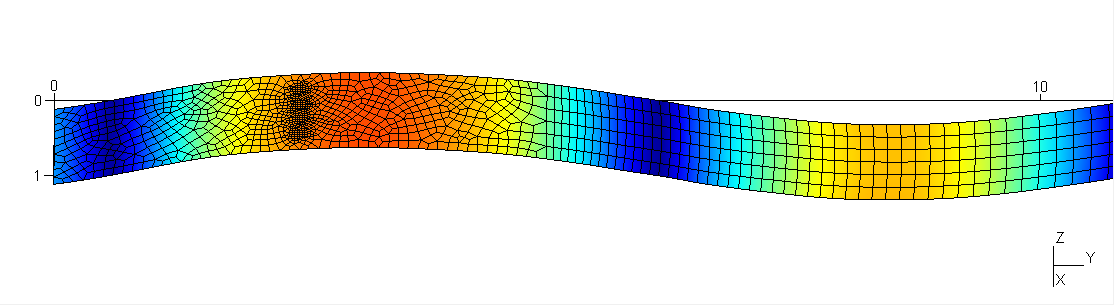
\includegraphics[width=1.0\textwidth,trim={0cm 0cm 0cm 0cm},clip]{Young/1E11/Dynamic.png}}



\end{frame}




\begin{frame}
\frametitle{Response of the plate for different Axial velocities(V) $m/s $}
\begin{figure}[h!]
\centering
\subfile{V_Pn2.tex}
%\caption{NAS277} \label{NAS277sch}
\end{figure}
\end{frame}

\begin{frame}
\frametitle{Response of the plate for different Thickness(t) $m$ }
\begin{figure}[h!]
\centering
\subfile{t_Pn2.tex}
%\caption{NAS277} \label{NAS277sch}
\end{figure}
\end{frame}




\begin{frame}
\frametitle{Response of the plate for different Densities($\rho$) $Kg/m^3$}
\begin{figure}[h!]
\centering
\subfile{Rho_Pn2.tex}
%\caption{NAS277} \label{NAS277sch}
\end{figure}
\end{frame}

\begin{frame}
\frametitle{Response of the plate for different Poisson's ratio ($\nu$)}
\begin{figure}[h!]
\centering
\subfile{Nu_Pn2.tex}
%\caption{NAS277} \label{NAS277sch}
\end{figure}
\end{frame}

\begin{frame}
\frametitle{Response of the plate for different Axial Tension (N) $N/m^2$}
\begin{figure}[h!]
\centering
\subfile{N_Pn2.tex}
%\caption{NAS277} \label{NAS277sch}
\end{figure}
\end{frame}

\begin{frame}
\frametitle{Response of the plate for different Young's modulus (E) $Pa$}
\begin{figure}[h!]
\centering
\subfile{Young_Pn2.tex}
%\caption{NAS277} \label{NAS277sch}
\end{figure}
\end{frame}



\begin{frame}
\frametitle{Response of the plate for different Young's modulus (E) with applied force}
\begin{figure}[h!]
\centering
\subfile{Young_for_Pn2.tex}
%\caption{NAS277} \label{NAS277sch}
\end{figure}
\end{frame}


\section{Mesh Dependency Test}


\begin{frame}


\begin{figure}[h!]
\centering
\begin{subfigure}{1\textwidth}
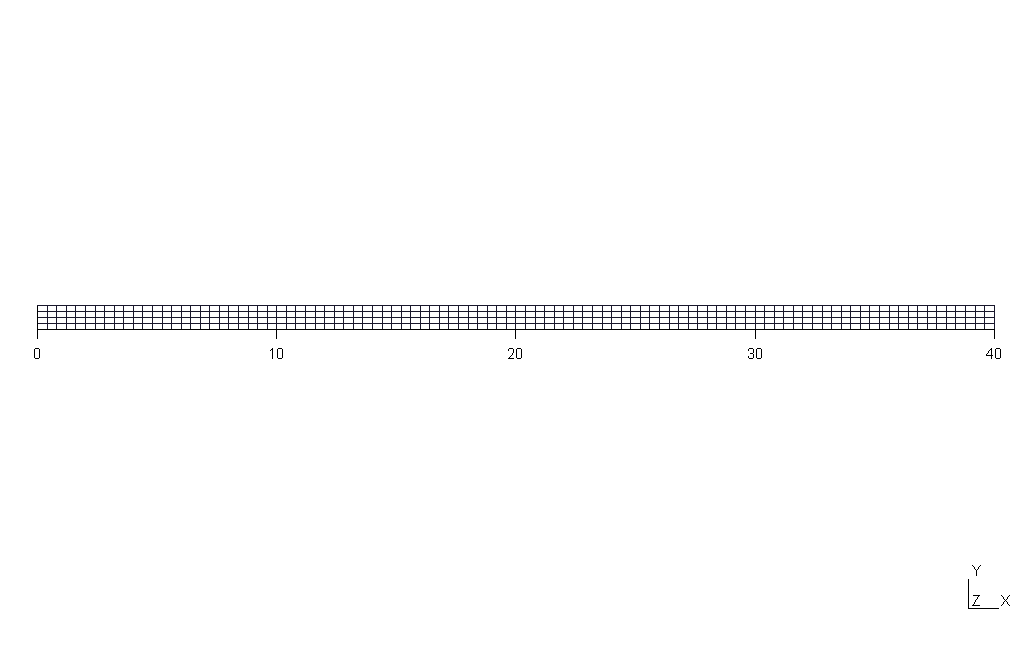
\includegraphics[width=\linewidth,trim={0.2cm 11cm 0.2cm 11cm},clip]{Mesh_Dependency/meshes/1.png}
\caption{Mesh : $1$ , No of Nodes = 505 }
\end{subfigure} \vfill
\begin{subfigure}{1\textwidth}
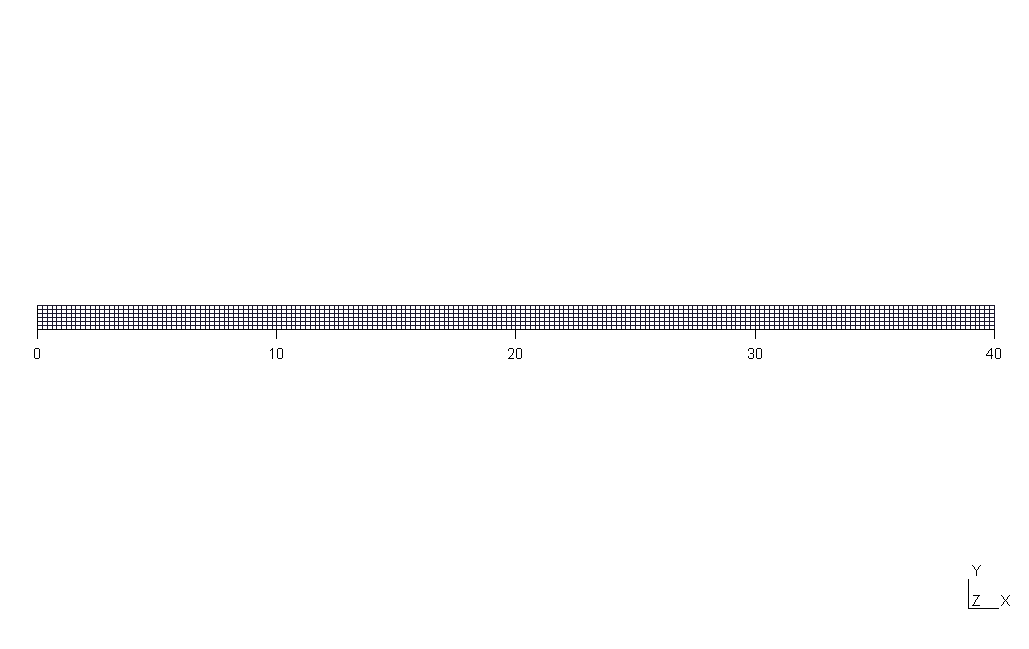
\includegraphics[width=\linewidth,trim={0.2cm 11cm 0.2cm 11cm},clip]{Mesh_Dependency/meshes/2.png}
\caption{Mesh : $2$ , No of Nodes = 1407}
\end{subfigure}\vfill
\begin{subfigure}{1\textwidth}
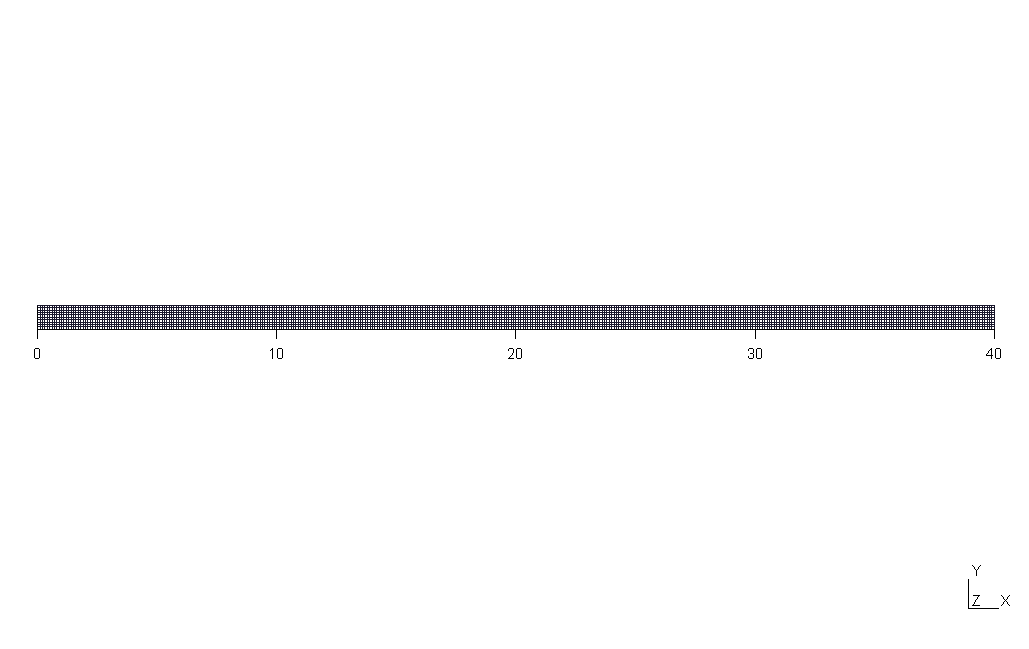
\includegraphics[width=\linewidth,trim={0.2cm 11cm 0.2cm 11cm},clip]{Mesh_Dependency/meshes/3.png}
\caption{Mesh : $3$ , No of Nodes = 4411}
\end{subfigure}\vfill
\begin{subfigure}{1\textwidth}
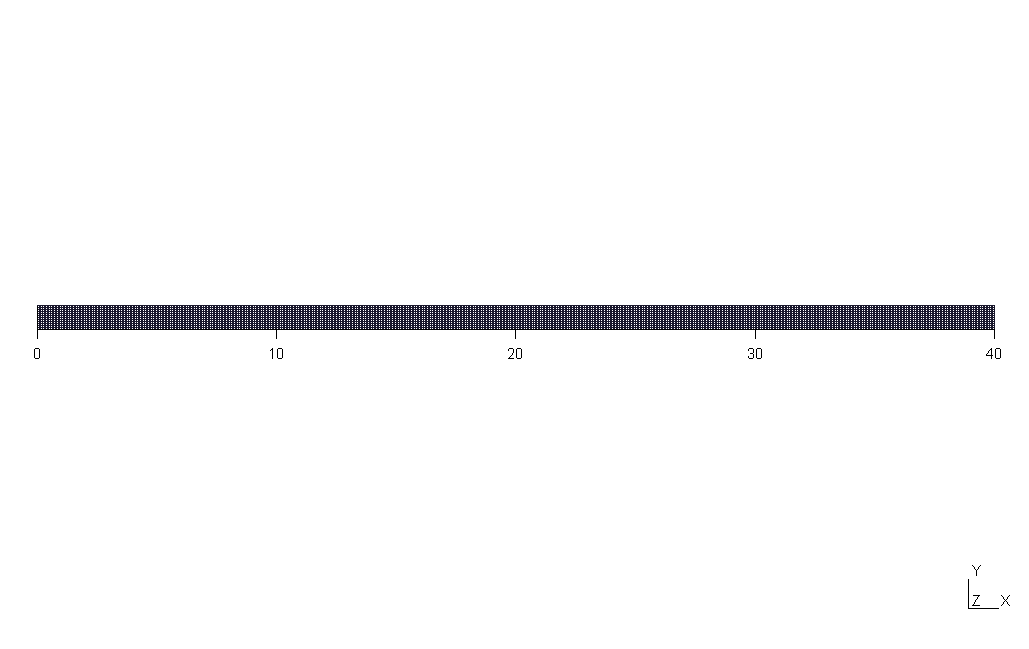
\includegraphics[width=\linewidth,trim={0.2cm 11cm 0.2cm 11cm},clip]{Mesh_Dependency/meshes/4.png}
\caption{Mesh : $4$ , No of Nodes = 7711}
\end{subfigure}\vfill
\begin{subfigure}{1\textwidth}
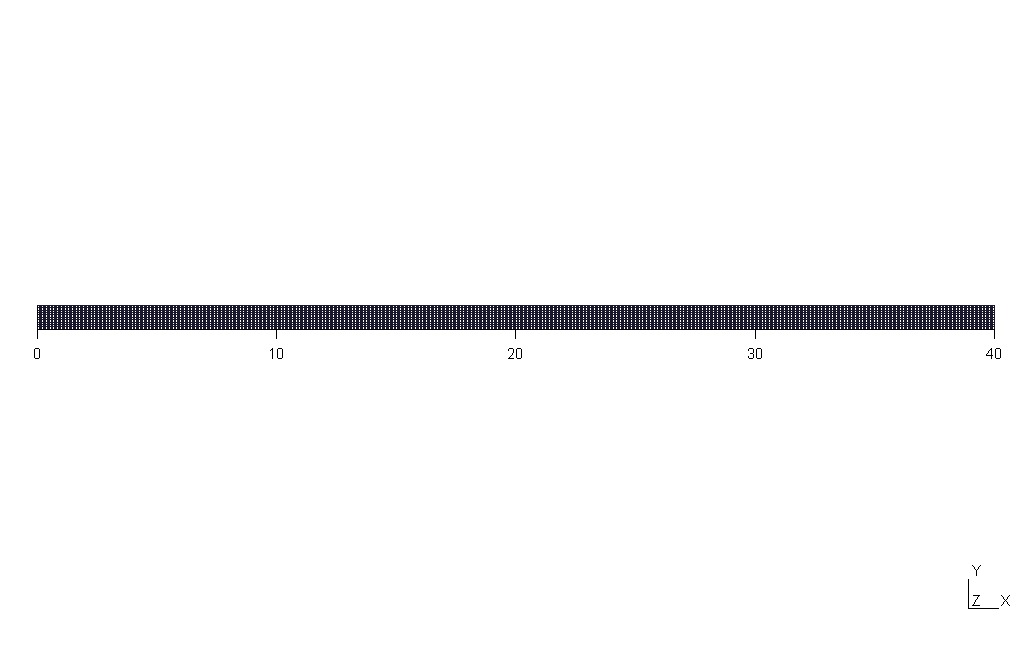
\includegraphics[width=\linewidth,trim={0.2cm 11cm 0.2cm 11cm},clip]{Mesh_Dependency/meshes/5.png}
\caption{Mesh : $5$ , No of Nodes = 7813}
\end{subfigure}

%\caption{Natural Modes of a rectangular strip}
\end{figure}

\end{frame}




\begin{frame}
\frametitle{Mesh Dependency test 1}
\begin{figure}[h!]
\centering
\subfile{Mesh_Dep.tex}
%\caption{NAS277} \label{NAS277sch}
\end{figure}
\end{frame}



%\includegraphics[width=\linewidth]{MeshDependency/2_0.png}
\begin{frame}


\begin{figure}[h!]
\centering
\begin{subfigure}{1\textwidth}
\includegraphics[width=\linewidth,trim={0.2cm 5.6cm 0.2cm 1cm},clip]{Mesh_Dependency/meshes/2_0.png}
\caption{Mesh : $2\_0$ , Skewness Ratio = 1}
\end{subfigure} \vfill
\begin{subfigure}{1\textwidth}
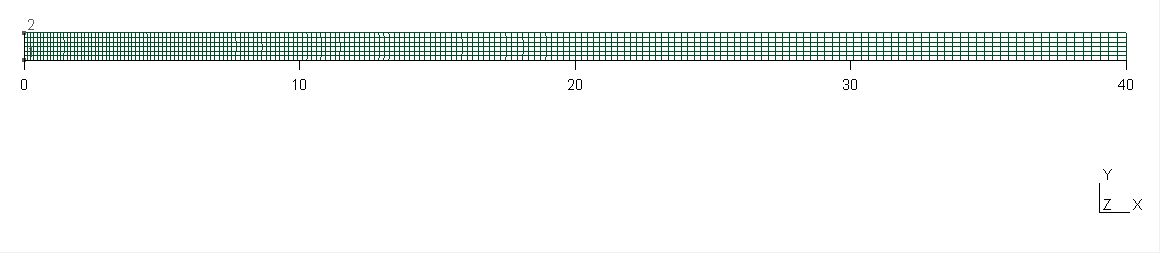
\includegraphics[width=\linewidth,trim={0.2cm 5.6cm 0.2cm 1cm},clip]{Mesh_Dependency/meshes/2_1.png}
\caption{Mesh : $2\_1$ , Skewness Ratio = 1.005}
\end{subfigure}\vfill
\begin{subfigure}{1\textwidth}
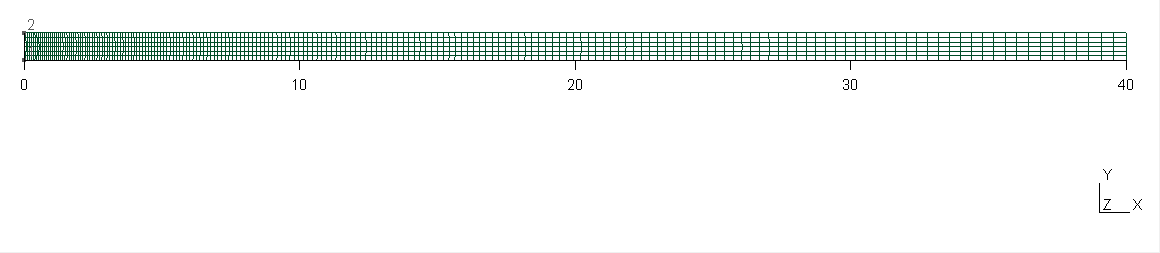
\includegraphics[width=\linewidth,trim={0.2cm 5.6cm 0.2cm 1cm},clip]{Mesh_Dependency/meshes/2_2.png}
\caption{Mesh : $2\_2$ , Skewness Ratio = 1.01}
\end{subfigure}\vfill
\begin{subfigure}{1\textwidth}
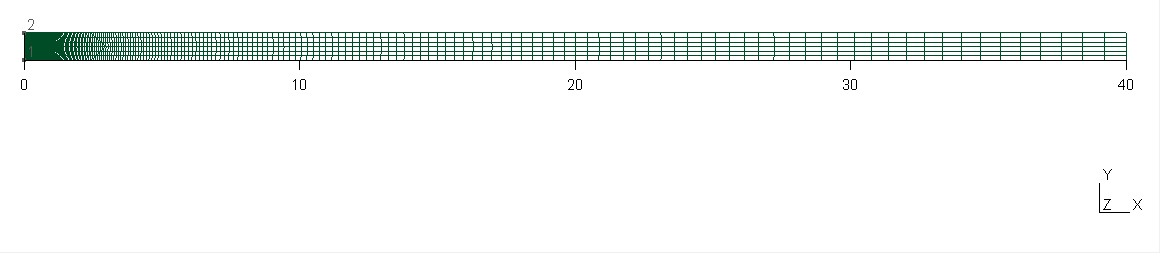
\includegraphics[width=\linewidth,trim={0.2cm 5.6cm 0.2cm 1cm},clip]{Mesh_Dependency/meshes/2_3.png}
\caption{Mesh : $2\_3$ , Skewness Ratio = 1.02}
\end{subfigure}\vfill
\begin{subfigure}{1\textwidth}
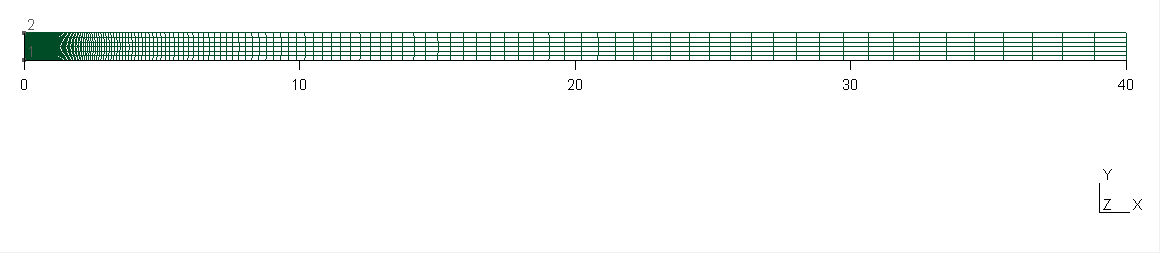
\includegraphics[width=\linewidth,trim={0.2cm 5.6cm 0.2cm 1cm},clip]{Mesh_Dependency/meshes/2_4.png}
\caption{Mesh : $2\_4$ , Skewness Ratio = 1.03}
\end{subfigure}

%\caption{Natural Modes of a rectangular strip}
\end{figure}

\end{frame}



\begin{frame}
\frametitle{Mesh Dependency test 2}
\begin{figure}[h!]
\centering
\subfile{Mesh_Dep1.tex}
%\caption{NAS277} \label{NAS277sch}
\end{figure}
\end{frame}


\begin{frame}
\begin{figure}[h!]
\centering

\begin{subfigure}{1\textwidth}

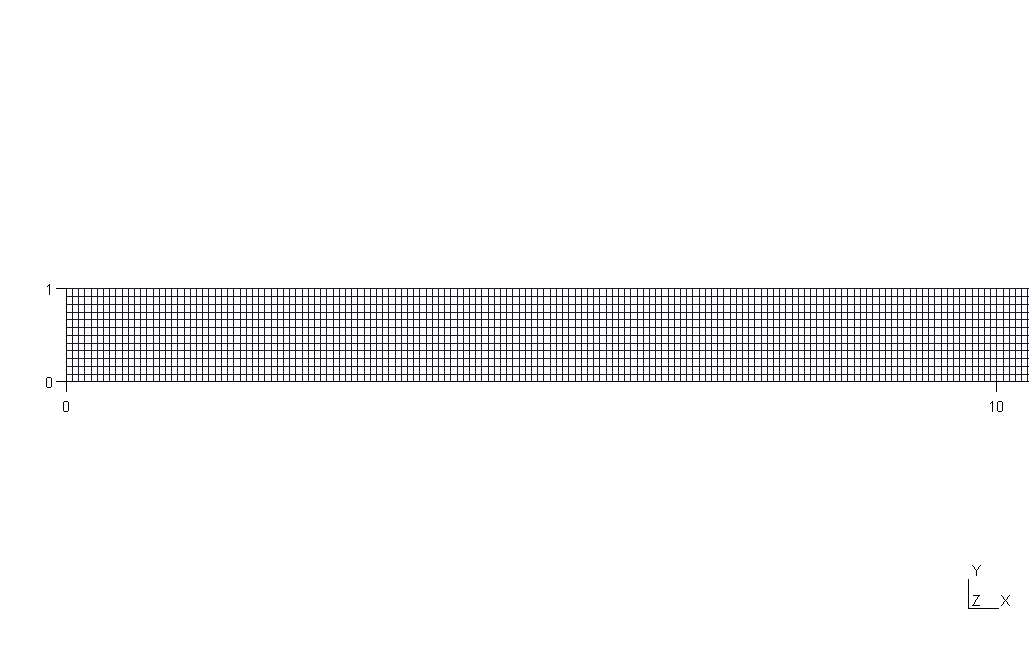
\includegraphics[width=\linewidth,trim={0cm 9cm 0cm 9cm},clip]{Mesh_Dependency/meshes/4_zoomed.png}
\caption{Mesh : $4$ , Nn = 7813 }

\end{subfigure} \vfill


\begin{subfigure}{1\textwidth}

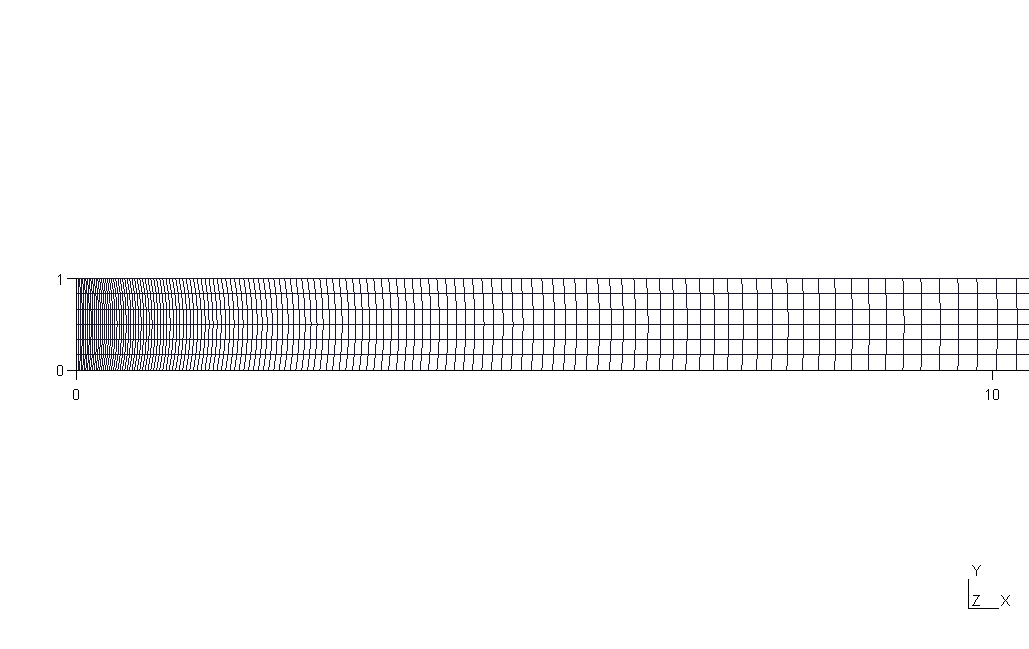
\includegraphics[width=\linewidth,trim={0cm 9cm 0cm 9cm},clip]{Mesh_Dependency/meshes/2_3_zoomed.png}
\caption{Mesh : $2\_3$ , Nn = 1407 }

\end{subfigure} \vfill

\begin{subfigure}{1\textwidth}

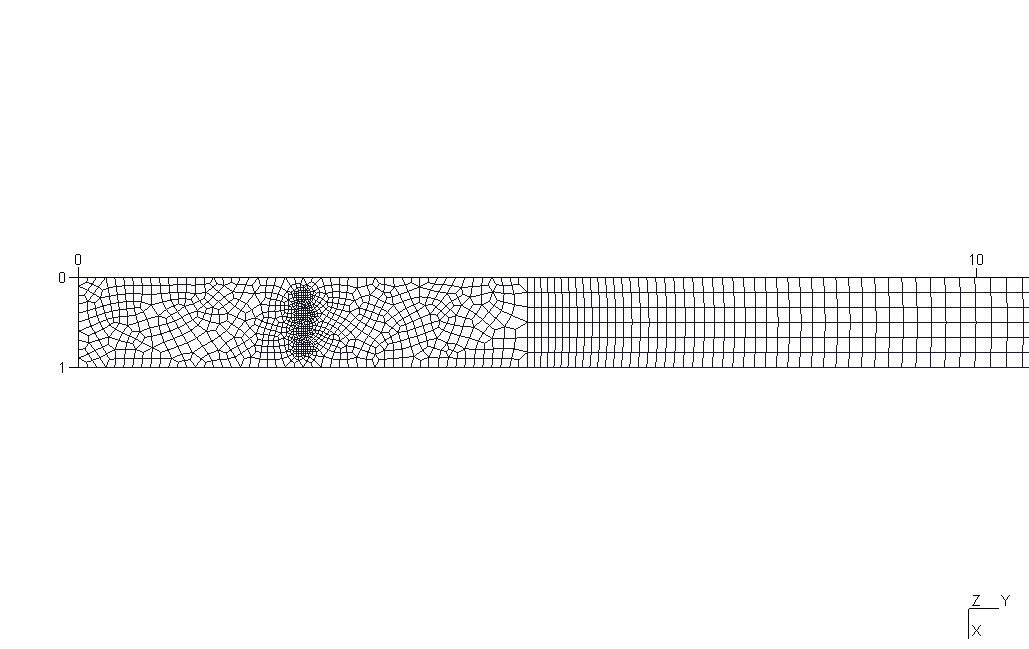
\includegraphics[width=\linewidth,trim={0cm 9cm 0cm 9cm},clip]{Mesh_Dependency/meshes/strip.png}
\caption{Mesh : strip , Nn = 1886 }

\end{subfigure} 


\end{figure}
\end{frame}


\begin{comment}
\begin{frame}
\frametitle{Mesh Dependency test 3}
\begin{figure}[h!]
\centering
\subfile{Mesh_Dep2.tex}
%\caption{NAS277} \label{NAS277sch}
\end{figure}
\end{frame}
\end{comment}

\section{Random displacement Load}
\begin{frame}
\frametitle{Strip with displacement from real world data }
\begin{columns}

\column{0.8\textwidth}

\pgfplotsset{width=9cm,height=3cm,compat=1.16}
\begin{tikzpicture}
\begin{axis}[
%title= Plot of W displacement VS Time,
axis x line = bottom,
axis y line = left,
xlabel={$Time (s)$},
ylabel={w at y=0},
xmin=0, xmax=5,
%minor y tick num=1,
%legend pos=outer north east,
%cycle list name = color list,
%transpose legend,
%legend columns=3,
%legend style={at={(0.5,-0.1)},anchor=north},
]

%\addplot table{PN2.txt};
%\addplot [blue] table{1E11/Dynamic_Rad_Pn2.txt};
\addplot [blue] table{RandomLoad/Load2.txt};
%\addlegendentry{$SR$ = 1, ST = 2s}


\end{axis}
\end{tikzpicture}



\pgfplotsset{width=9cm,height=3cm,compat=1.16}
\begin{tikzpicture}
\begin{axis}[
%title= Plot of W displacement VS Time,
axis x line = bottom,
axis y line = left,
xlabel={$Time (s)$},
ylabel={w at y=0.5},
xmin=0, xmax=5,
%minor y tick num=1,
%legend pos=outer north east,
%cycle list name = color list,
%transpose legend,
%legend columns=3,
%legend style={at={(0.5,-0.1)},anchor=north},
]

%\addplot table{PN2.txt};
%\addplot [blue] table{1E11/Dynamic_Rad_Pn2.txt};
\addplot [blue] table{RandomLoad/Load1.txt};
%\addlegendentry{$SR$ = 1, ST = 2s}


\end{axis}
\end{tikzpicture}



\pgfplotsset{width=9cm,height=3cm,compat=1.16}
\begin{tikzpicture}
\begin{axis}[
%title= Plot of W displacement VS Time,
axis x line = bottom,
axis y line = left,
xlabel={$Time (s)$},
ylabel={w at y=1},
xmin=0, xmax=5,
%minor y tick num=1,
%legend pos=outer north east,
%cycle list name = color list,
%transpose legend,
%legend columns=3,
%legend style={at={(0.5,-0.1)},anchor=north},
]

%\addplot table{PN2.txt};
%\addplot [blue] table{1E11/Dynamic_Rad_Pn2.txt};
\addplot [blue] table{RandomLoad/Load3.txt};
%\addlegendentry{$SR$ = 1, ST = 2s}


\end{axis}
\end{tikzpicture}

\column{0.2\textwidth}
\href{run:RandomLoad/Dynamic_Rad1.mpg}{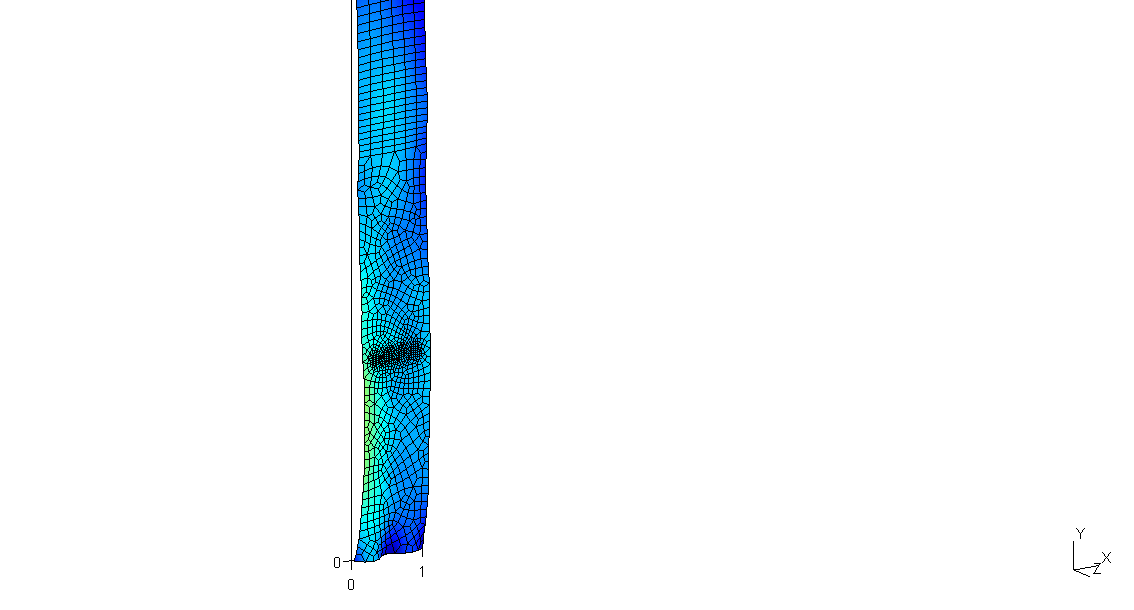
\includegraphics[width=1.0\textwidth,trim={11cm 0cm 22cm 0cm},clip]{RandomLoad/Dynamic_Rad1.png}}
\end{columns}
\end{frame}

\section{Pure Twisting Deformation}

\begin{frame}
\frametitle{Plate twisted in one end with axial stress = 3E7 $N/m^2$  }

%\includegraphics[width=\linewidth,trim={0cm 0cm 0cm 0cm},clip]{N2/0E1/static.png}

\href{run:N2/3E7/Dynamic.mpg}{\includegraphics[width=\linewidth,trim={0cm 0cm 0cm 0cm},clip]{N2/0E1/static.png}}
\end{frame}

\begin{comment}

\begin{frame}
\frametitle{Plate twisted in one end with axial stress = 100 $N/m^2$  }

\includegraphics[width=\linewidth,trim={0cm 0cm 0cm 0cm},clip]{N2/1E2/static.png}

\end{frame}

\begin{frame}
\frametitle{Plate twisted in one end with axial stress = 1000 $N/m^2$  }

\includegraphics[width=\linewidth,trim={0cm 0cm 0cm 0cm},clip]{N2/1E3/static.png}

\end{frame}

\begin{frame}
\frametitle{Plate twisted in one end with axial stress = 10000 $N/m^2$  }

%\includegraphics[width=\linewidth,trim={0cm 0cm 0cm 0cm},clip]{N2/1E4/static.png}

\href{run:N2/3E7/Dynamic.mpg}{\includegraphics[width=\linewidth,trim={0cm 0cm 0cm 0cm},clip]{N2/1E4/static.png}}

\end{frame}

\end{comment}

\begin{frame}
Thank you for your attention!!!
\end{frame}

\end{document}
